\documentclass{article}

\usepackage{amsmath}
\usepackage{amsthm}
\usepackage{amssymb}
\usepackage{bbm}
\usepackage{fancyhdr}
% \usepackage{listings}
\usepackage{cite}
\usepackage{graphicx}
\usepackage{enumitem}
\usepackage{courier}
\usepackage[pdftex,colorlinks=true, urlcolor = blue]{hyperref}


\oddsidemargin 0in \evensidemargin 0in
\topmargin -0.5in \headheight 0.25in \headsep 0.25in
\textwidth 6.5in \textheight 9in
\parskip 6pt \parindent 0in \footskip 20pt

% set the header up
\fancyhead{}
\fancyhead[L]{Stanford Aeronautics \& Astronautics}
\fancyhead[R]{Winter 2019}

%%%%%%%%%%%%%%%%%%%%%%%%%%
\renewcommand\headrulewidth{0.4pt}
\setlength\headheight{15pt}

\usepackage{xparse}
\NewDocumentCommand{\codeword}{v}{%
\texttt{\textcolor{blue}{#1}}%
}

\usepackage{xcolor}
\setlength{\parindent}{0in}

\title{CS224N \\ Assignment 2}
\author{Name: Oscar      \\ SUID: 05735451}
\date{}

\begin{document}

\maketitle
\pagestyle{fancy} 

\section*{Problem 1: Understanding word2vecl}
\begin{enumerate}[label=(\roman*)]
\item{ A}
	The proof that these two are equal should be 
%	-log(\dfrac{exp(u_o^Tv_c)}{{\sum}exp(u_o^Tv_c)}) = 
\[
	- {\sum}y_wlog(\hat{y}_w) = -log(\hat{y}_o)
\]
This is true because $y_w$ will be equal to zero whenever w is not o. This means that the summation will, in practical terms, disappear, making the above expression true.  

\item {B: $\dfrac{dj}{dv_c}$}
\[
J = -log(\dfrac{exp(u_o^Tv_c)}{{\sum}exp(u_o^Tv_c)})  = -log(exp(u_o^Tv_c)) + log({\sum}exp(u_o^Tv_c))
\]
\[
\dfrac{dj}{dv_c} = -u_0^T + \dfrac{1}{{\sum}exp(u_o^Tv_c)}{\sum}exp(u_o^Tv_c)u_o^T
\]
\[
\dfrac{dj}{dv_c} = -u_0^T + {\sum}\hat{y}u_w =\sum_wu_w(\hat{y}_w - y_w)
\]

\item {C: $\dfrac{dj}{du}$}\\
\\
o = w
\[
	J = -log(\dfrac{exp(u_o^Tv_c)}{{\sum}exp(u_o^Tv_c)})  = -log(exp(u_o^Tv_c)) + log({\sum}exp(u_o^Tv_c))
\]
\[
	\dfrac{dj}{du} = -v_c^T + \dfrac{1}{{\sum}exp(u_o^Tv_c)}{\sum}exp(u_o^Tv_c)v_c^T = -v_c^T + \hat{y}v_c
\]
o $\neq$ w
\[
	\dfrac{dj}{du} = \dfrac{1}{{\sum}exp(u_o^Tv_c)}{\sum}exp(u_o^Tv_c)v_c^T =  \hat{y}_wv_c
\]

\item{D}
\[
	\dfrac{d\sigma}{dx} = -(1 + e^{-z})^{-2}e^{-z} = \dfrac{=e^{-z}+1-1}{(1 + e^{-z})^{2}}
\]
\[
	\dfrac{d\sigma}{dx} = \dfrac{1}{1 + e^{-z}} - \dfrac{1}{1+e^{-z}}^2 = \sigma(1-\sigma)
\]

\item{E}
\[
	J = -log(\sigma(u_o^Tv_c)) - \sum^Klog(\sigma(-u_k^Tv_c))
\]
\[
	\dfrac{dJ}{v_c} = -\dfrac{1}{\sigma(u_o^Tv_c)}\sigma(u_o^Tv_c)(1- \sigma(u_o^Tv_c))u_o - \sum^K\dfrac{1}{\sigma(-u_k^Tv_c)}\sigma(-u_k^Tv_c)(1- \sigma(-u_k^Tv_c))(-u_k)
\]
\[
	\dfrac{dJ}{v_c} = -(1- \sigma(u_o^Tv_c))u_o - \sum^K(1- \sigma(-u_k^Tv_c))(-u_k)
\]
\[
	\dfrac{dJ}{u_o} = -\dfrac{1}{\sigma(u_o^Tv_c)}\sigma(u_o^Tv_c)(1- \sigma(u_o^Tv_c))v_c^T
\]
\[
	\dfrac{dJ}{u_o} = -(1- \sigma(u_o^Tv_c))v_c^T
\]
\[
	\dfrac{dJ}{u_k} = \dfrac{1}{\sigma(-u_k^Tv_c)}\sigma(-u_k^Tv_c)(1- \sigma(-u_k^Tv_c))-(v_c)
\]
\[
	\dfrac{dJ}{u_k} = (1- \sigma(-u_k^Tv_c))-v_c
\]

\item{F}
\[
	\dfrac{dJ}{dU} = \sum^m\dfrac{dJ}{dU}
\]
\[
	\dfrac{dJ}{dv_c} = \sum^m\dfrac{dJ}{dv_c}
\]

\[
	\dfrac{dJ}{dv_w} = \sum^m\dfrac{dJ}{dv_w}
\]

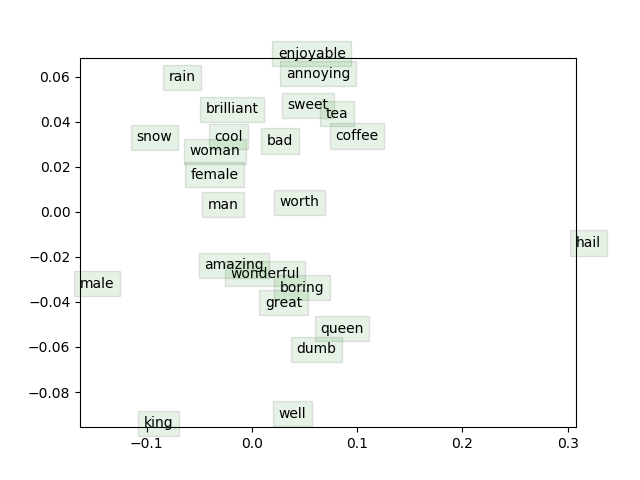
\includegraphics{word_vectors.png}
This plot is interesting because we can see certain associations between word vectors. There's a group of adjectives grouped in the center. It's also interesting seeing the associations between man and king and queen and women. t
\end{enumerate}


\end{document}
